%%%%%%%%%%%%%%%%%%%%%%%%%%%%%%%%%%%%%%%%%%%%%%%%%%%%
\section{Informed Plan Selection}\label{sec:coverage-intro}
%%%%%%%%%%%%%%%%%%%%%%%%%%%%%%%%%%%%%%%%%%%%%%%%%%%%

The first part of this paper addresses the task of determining when decisions along the active execution trace may be considered \textit{informed enough} for outcomes to be included as learnable instances for each \dt in that trace. For this we contrast two schemes, \CL\ and \BUL\ - and show that the conservative \BUL\ approach delivers more robust performance than the simpler \CL\ approach for the cases considered. For both approaches, the same probabilistic function $E$ (or exploration strategy) was used to make the plan selection at each junction of the active execution trace.

In subsequent work we keep the \CL\ and \BUL\ recording methods constant, and adjust the probabilistic plan selection function $E$ to evaluate the impact on the learning outcome. Motivated by the polarity between the two approaches, we consider if an informed probabilistic selection function $E'$ may be constructed to yield a "middle ground" approach that applies better in the general case. This would be valuable since if a \CL+$E'$-based approach yields comparable performance to any \BUL+$E^*$-based approach, then the former is preferred as \CL\ is much simpler than \BUL. Interestingly we find that such a formulation is possible and that an informed exploration strategy that leverages both the domain knowledge (inherent in the goal-plan tree hierarchy) as well as the ongoing learning (agent's experience so far) can combine the benefits of both \CL\ and \BUL.

We start by quantifying the quality of (or our \textit{confidence} in) the hypotheses of a \dt for a unknown but learnable subspace $S$ of worlds $[W_1 \ldots W_n]$. At the beginning of a run we have no learnable instances and for a given goal-plan tree node $T$ our probability of success $p_T(W)$ in world $W \in S$ is given by the default probability $P_d=0.5$. After the first instance is recorded, the \dt will generalise the result to the full space of $S$ (i.e. $\forall W \in S$) leading to likely \textit{misclassification}. Intuitively we know that as more and more $W \in S$ are witnessed and recorded, the \dt's classification over $S$ will improve. Our two approaches may be described in terms of confidence as follows: \CL\ always assumes full confidence in the \dt but suffers from misclassification errors (that are eventually rectified through subsequent learning from misinformed choices); \BUL\ uses the static $\epsilon$ and $k$ values to determine the boundary for our confidence in the \dt (with the trade-off that for the period of no confidence the best we can do is use $P_d$).

One way to improve this situation is to instead compute a smooth transition from zero-confidence in the \dt classification to full-confidence, based on experience. We identify two orthogonal properties, \textit{choices} and \textit{subspace} that are integral to informed decision making by the learning nodes in our agent. Choices refer to the set of all statically computable execution paths \textit{below} a goal node in the goal-plan tree hierarchy. Subspace refers to the set of all worlds that are learnable for the \dt at that node. Defined in those terms, we label a \dt \textit{not informed} if no choices have been recorded in any world of the subspace, or \textit{fully informed} when all choices have been covered in every world of the subspace. In fact, we can construct a measure of our confidence in the \dt based on the degree of \textit{coverage} of all choices in all subspace associated worlds.

\begin{equation}
\label{eqn:coverage}   
E': p'_T(W)= P_d + \left[  c_T(S) *  \left( p_T(W) - P_d \right)  \right]
\end{equation}

Equation \ref{eqn:coverage} shows how a confidence measure based on coverage may be used to modify the final plan selection probability. The idea is to bias the \dt classification (probability of success) of world $W$ in node $T$ given by $p_T(W) \in [0 \ldots 1]$ with the coverage $c_T(S) \in [0 \ldots 1]$ of subspace $S$ given $W \in S$. Initially the coverage is zero, so the revised probability $p'_T(W) = P_d$ the default probability of success. As coverage $\rightarrow 1$, the revised probability $p'_T(W) \rightarrow p_T(W)$ the \dt classification. This gives a progressive transition to the \dt classification as more experience is acquired (Figure \ref{fig:coverage-surface}).

\begin{figure}[ht]
   \centering
   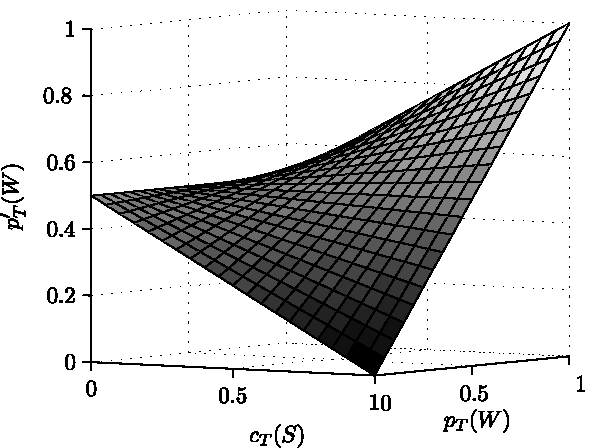
\includegraphics[width=\columnwidth]{figs/coverage-surface}
   \caption{How coverage impacts \dt classification}
   \label{fig:coverage-surface}
\end{figure}


The coverage $c_T(S)$ itself is calculated and stored each time a result is recorded for node $T$. The calculation is performed in turn for each node in the active execution trace starting at the leaf node where the failure occurred, and the coverage is updated progressively up the tree hierarchy. Full coverage at a node $T$ has a computation cost of $C(T)*|S|$ where $C(T)$ is the total number of choices below $T$ and $|S|$ is the number of worlds in the subspace. Practically however, it costs significantly less since choices below $T$ are effectively AND/OR trees, and each time an AND node fails the subsequent nodes are not tried and are assumed covered for that world. The full memory cost for a subspace with $n$ boolean attributes is $2^a*C(T)$ however we only require $2^a$ for the implementation since we do not keep track of each individual path below $T$ but only how many distinct paths below $T$ have been tried in a given world. The only unknown in the coverage calculation is $S$ since we do not know upfront the subspace to be learnt. A fairly useful estimate of $c_T(S)$ for practical use can however be constructed by averaging the individual coverages $c_T(W_i)$ of all previously seen worlds at node $T$. 


\begin{figure}[ht]
\centering
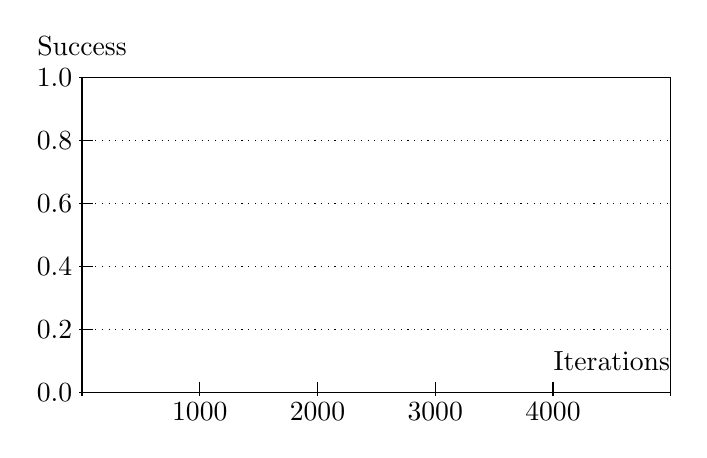
\begin{tikzpicture}[x=0.0015cm,y=4cm]
    % Draw the axes and grid lines
    \draw[-] (0,0) -- (0,1) -- (5000,1) -- (5000,0) -- cycle; 
    \draw[-,thin, dotted, ystep=0.2, xstep=5000] (0,0) grid (5000,1);
    \foreach \x in {0,1000,...,5000}  \draw [-,xshift=0](\x,4pt) -- (\x,-1pt);
    \foreach \y in {0.0,0.2,0.4,0.6,0.8,1.0}  \draw [-,yshift=0](4pt,\y) -- (-1pt,\y);
    \foreach \x/\xtext in {1000/1000, 2000/2000, 3000/3000, 4000/4000} \node at (\x,0) [below] {$\xtext$};
    \foreach \y/\ytext in {0.0,0.2,0.4,0.6,0.8,1.0}  \node at (0,\y) [left] {$\ytext$};
    \node at (0,1.1) {Success};
    \node at (4500,0.1) {Iterations};
    \draw[-] plot[mark=square,mark size=2,mark options={color=black}] 
			file {data/test05v5gm.CC.tikzdata};
    \draw[-,thin,densely dashed,gray] plot[mark=triangle,gray,mark size=3,mark options={color=gray}] 
			file {data/test05v5gm.CP.tikzdata};
    \draw[-] plot[mark=diamond,mark size=3,mark options={color=black}] 
			file {data/test05v5gm.SC.tikzdata};
    \draw[-,thin,densely dashed,gray] plot[mark=o,gray,mark size=2,mark options={color=gray}] 
			file {data/test05v5gm.SP.tikzdata};

\end{tikzpicture}
\caption{$\T_2$}
\end{figure}


\begin{figure}[ht]
\centering
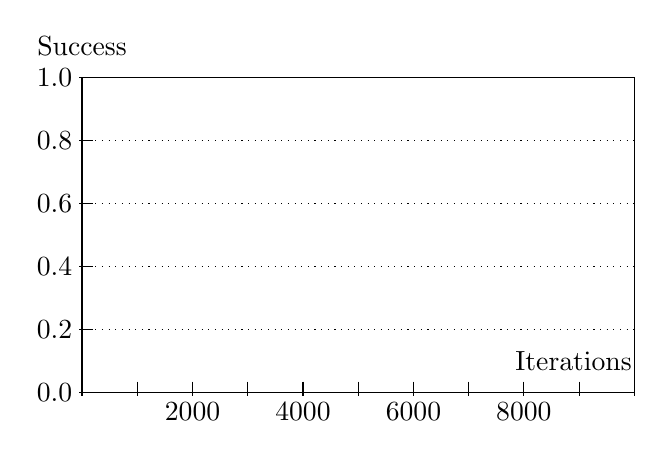
\begin{tikzpicture}[x=0.0007cm,y=4cm]
    % Draw the axes and grid lines
    \draw[-] (0,0) -- (0,1) -- (10000,1) -- (10000,0) -- cycle; 
    \draw[-,thin, dotted, ystep=0.2, xstep=10000] (0,0) grid (10000,1);
    \foreach \x in {0,1000,...,10000}  \draw [-,xshift=0](\x,4pt) -- (\x,-1pt);
    \foreach \y in {0.0,0.2,0.4,0.6,0.8,1.0}  \draw [-,yshift=0](4pt,\y) -- (-1pt,\y);
    \foreach \x/\xtext in {2000/2000, 4000/4000, 6000/6000, 8000/8000} \node at (\x,0) [below] {$\xtext$};
    \foreach \y/\ytext in {0.0,0.2,0.4,0.6,0.8,1.0}  \node at (0,\y) [left] {$\ytext$};
    \node at (0,1.1) {Success};
    \node at (8900,0.1) {Iterations};
    \draw[-] plot[mark=square,mark size=2,mark options={color=black}] 
			file {data/testMultiSolutionsR.CC.tikzdata};
    \draw[-,thin,densely dashed,gray] plot[mark=triangle,gray,mark size=3,mark options={color=gray}] 
			file {data/testMultiSolutionsR.CP.tikzdata};
    \draw[-] plot[mark=diamond,mark size=3,mark options={color=black}] 
			file {data/testMultiSolutionsR.SC.tikzdata};
    \draw[-,thin,densely dashed,gray] plot[mark=o,gray,mark size=2,mark options={color=gray}] 
			file {data/testMultiSolutionsR.SP.tikzdata};

\end{tikzpicture}
\caption{$\T_4$}
\end{figure}


